\section{Результати роботи програми}

Для верифікації правильності роботи розроблених алгоритмів, контролю стану 
об'єктів та перевірки механізмів інкапсуляції було здійснено запуск програми 
в єдиному циклі збирання середовища VS Code. На рисунку~\ref{fig:terminal_lab2} 
представлено фінальний вивід результатів у термінал Windows PowerShell.

\begin{figure}[H]
    \centering
    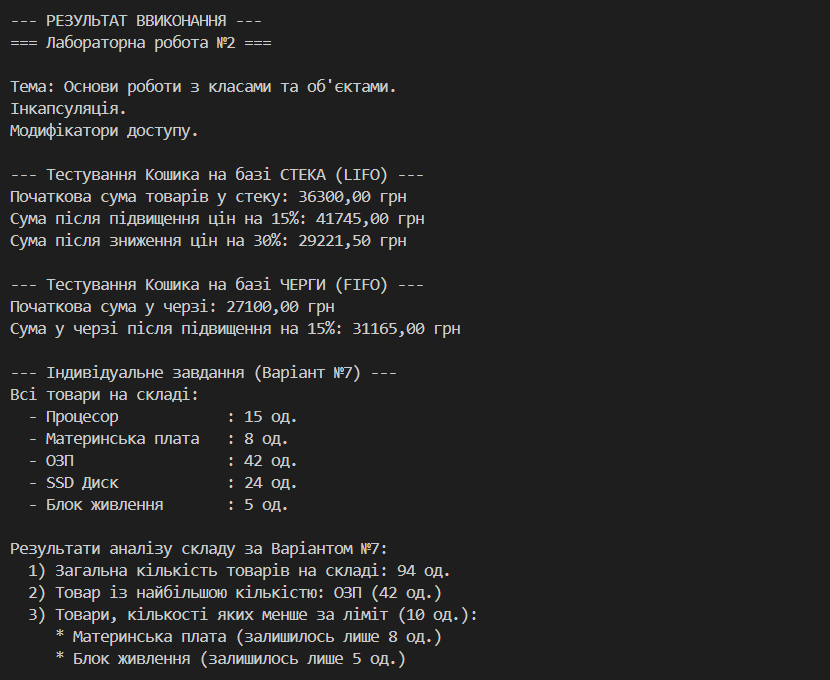
\includegraphics[width=0.95\textwidth]{screenshots/terminal_output.png}
    \caption{Вигляд терміналу після успішного виконання та тестування програми.}
    \label{fig:terminal_lab2}
\end{figure}

На основі отриманих даних терміналу (рис.~\ref{fig:terminal_lab2}) проведено покроковий 
аналіз виконання технічного завдання:
\begin{enumerate}
    \item \textbf{Тестування Кошика на базі Стека (\texttt{StackCart}):} 
    При ініціалізації п'ятьма базовими товарами загальна сума склала \texttt{36300.00 грн}. 
    Після надсилання об'єктам повідомлення \texttt{raiseAllPrices(15.0f)} сума успішно збільшилась 
    на $15\%$ і склала \texttt{41745.00 грн}. 
    Подальше зниження цін усіх товарів у стеку на $30\%$ через метод \texttt{cutAllPrices(30.0f)} 
    продемонструвало коректну зміну стану об'єктів — фінальна сума зафіксована на 
    рівні \texttt{29221.50 грн}.
    
    \item \textbf{Тестування сокрыття реалізації (\texttt{QueueCart}):}
    Зміна внутрішньої структури даних на кільцеву чергу (\texttt{FIFO}) при повному 
    збереженні зовнішнього інтерфейсу методів підтвердила успішність застосування інкапсуляції. 
    Об'єкти додавалися та розраховувалися безпомилково, видаючи аналогічні математичні 
    результати для початкових тестів (\texttt{27100.00 грн} та \texttt{31165.00 грн} після 
    підвищення цін).
    
    \item \textbf{Аналіз складського обліку (Індивідуальний Варіант №7):}
    Компонент \texttt{WarehouseManager} провів лінійний аналіз паралельних масивів даних. 
    Програма безпомилково розрахувала загальну кількість одиниць техніки на складі (\texttt{94 од.}), 
    визначила лідера за обсягом залишків (товар «ОЗП» — \texttt{42 од.}) та здійснила фільтрацію 
    дефіцитних позицій за заданим лімітом у \texttt{10 од.}, вивівши у консоль товари 
    «Материнська плата» (\texttt{8 од.}) та «Блок живлення» (\texttt{5 од.}).
\end{enumerate}
